\documentclass[a4paper,12pt]{jsreport}
\usepackage{bm}
\usepackage[dvipdfmx]{graphicx}
\usepackage{ascmac}
\usepackage{amsthm}
\usepackage{amsmath, amssymb}
\usepackage{listings, jlisting}


\lstset{
  language={Python}, % 言語の指定
  basicstyle={\ttfamily},
  identifierstyle={\small},
  keywordstyle={\small\bfseries},
  ndkeywordstyle={\small},
  stringstyle={\small\ttfamily},
  frame={tb},
  breaklines=true,
  columns=[l]{fullflexible},
  numbers=left,
  xrightmargin=0zw,
  xleftmargin=3zw,
  numberstyle={\scriptsize},
  stepnumber=1,
  numbersep=1zw,
  lineskip=-0.5ex
}

\theoremstyle{definition}
\newtheorem{theorem}{定理}
\newtheorem{definition}[theorem]{定義}
\newtheorem{prop}{命題}
\newtheorem{algorithm}{アルゴリズム}

\title{2020年度\\卒業論文\\ \  \\強化学習による最適観光ルート推定の研究}
\author{統計ファイナンス研究室\\
山口真哉\\
学籍番号:1116179036}
\date{2021年1日6日}

\begin{document}
\maketitle
\tableofcontents

\chapter{はじめに}
交通手段やSNSの発展により,思いったらすぐに旅行ができるようになってきている.しかし,旅行で行きたい観光地は高々数個で時間を持て余してしまうようなケースが少なからず存在する.そのようなニーズに応えるべくユーザーの条件を満たしている最適観光ルートの推定を強化学習を用いて行う.本研究で構築するモデルは,行きたい場所,合計の所要時間,始点,終点などが独自に設定可能だが,他の制約条件を加えても同様に学習できるようなモデルを提案する.




\chapter{グラフ理論}
この章の内容は、渡邊先生の離散数学の授業を元に記録した講義ノートの定義を使う.
\section{定義}
\begin{definition}[無向グラフ]
    有限集合$V=\{v_1,v_2,\ldots,v_n\}$と有限集合$E=\{e_1,e_2,\ldots,e_n\}\subset V^2$を考える.このとき,2つの集合の組$G=(V,E)$を無向グラフという.集合$V$の要素をグラフ$G$の頂点,集合$E$の要素を$G$の辺という.また,$e=\{u,v\}\in E$であるとき,$u$と$v$は隣接するという.
\end{definition}
\begin{definition}[部分グラフ]
    無向グラフ$G=(V,E),G'=(V',E')$について,$V\subset V',E\subset E'$であるとき, $G$は$G'$の部分グラフという.
\end{definition}
\begin{definition}[道,\ path]
    無向グラフ$G=(V,E)$,$G$の互いに異なる頂点列$P=(v_1,v_2,\ldots, v_{k+1})$とする.
    \begin{equation}
        V'=\{v_i|\ i=1,2,\ldots,k+1\}
    \end{equation}
    \begin{equation}
        E'=\{\{v_i,v_{i+1}\}\in E\ |\ i=1,2,\ldots,k\}
    \end{equation}
    としたとき$G'=(V',E')$を$G$の長さ$k$の道(path)という.特に,$s=v_1,\ t=v_{k+1}$とすると,$G'$を$s-t$ pathという.
\end{definition}
\begin{definition}[辺次数]
    $G=(V,E)$を無向グラフとする.そのとき,$v\in V$に対して,$v$に隣接する辺の集合を$\delta(v)$で表す.このとき,$\deg_G(v)=|\delta(v)|$を頂点$ v$の辺次数と呼ぶ.
\end{definition}
\section{グラフの表現}
$G=(V,E)$を無向グラフ,$n=|V|$とする.$w:E\to \mathbb{R}$を重み関数とする.$n$次正方行列$A=A(G)=a_{ij}$を
\begin{eqnarray}
    a_{ij}=
    \begin{cases}
        & w(e)\ (e=\{v_i,v_j\}\in E)\\
        & \infty\ \ \ \ ({\rm otherwise})
    \end{cases}
\end{eqnarray}
で定義し$A(G)$を無向グラフの隣接行列という.\\
隣接行列でグラフを表現する場合,2頂点間に辺があるか否かが定数時間で判定できるが,常に$O(|V|^2)$のメモリを消費する.道のように辺の数が少ない疎グラフの場合,隣接行列のほとんどが$\infty$で埋まることになる.\\ \\
集合の列$A=A(G)=a_v$を
\begin{equation}
    a_v=\{(u,w(e))\ |\ u\in V,\ e=\{u,v\}\in E \})
\end{equation}
とする.$A(G)$を隣接リストという.\\
このとき$O(|V|+|E|)$のメモリしか消費しない.



\chapter{強化学習}
学習に用いた強化学習の理論を記す.\\
環境とは行動と行動の応じた状態の変化が定義されており,ある状態への到達に対して報酬が与えられる空間のことである.強化学習では教師あり学習や教師なし学習とは異なり,データを与えるのではなく環境を与える.強化学習のモデル(agent)は状態を受け取り行動を出力する関数で,与えられた環境においてエピソード全体の報酬の総和を最大化するようにパラメータを調整する.
\section{強化学習の問題設定} 
強化学習において与えられた環境は「遷移先の状態は直前の状態とそこでの行動にのみ依存する.報酬は直前の状態と遷移先に依存する」ということを仮定する.この性質をマルコフ性と呼び,マルコフ性を持つ環境をマルコフ決定過程(MDP)と呼ぶ.MDPの構成要素は以下の4つである.\\
$s$ : 状態,$a$ : 行動,$T(s,a)$ : 状態遷移の確率,$R(s_t,s_{t+1})$ : 即時報酬\textbf{}
\begin{figure}[h]
    \centering
    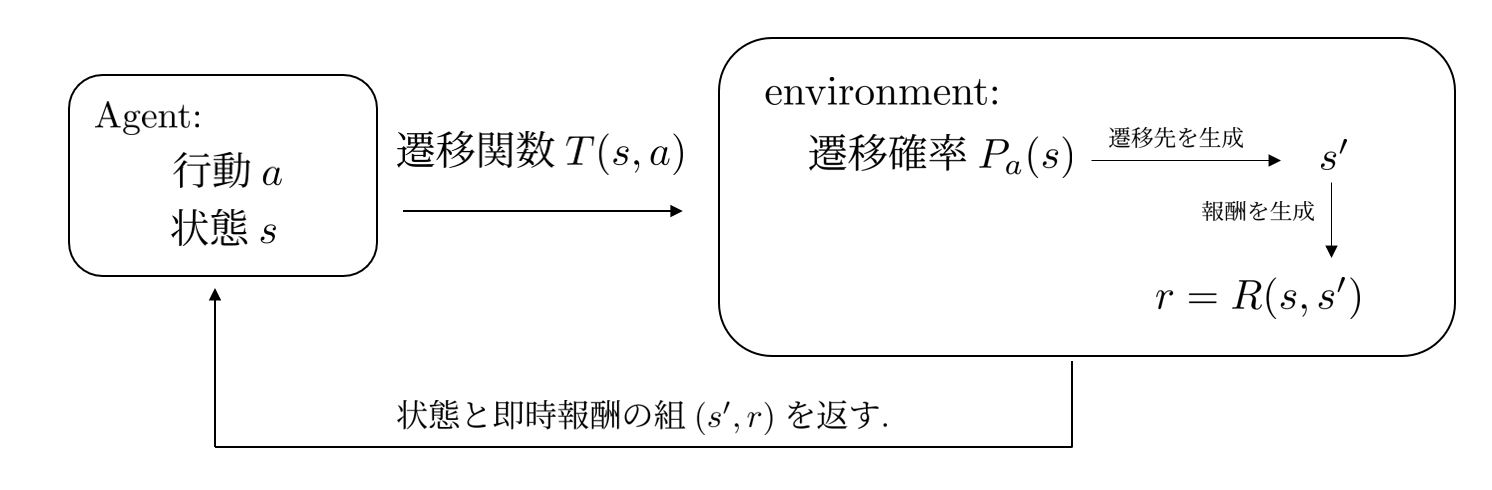
\includegraphics[width=10cm]{MDP.png}
    \caption{マルコフ決定過程の図式}
    \label{fig:MDP}
\end{figure}
\clearpage

MDPにおける報酬の総和は即時報酬の総和で定義される.エピソードの終了時刻を$T$としたとき,時刻$t$における報酬の総和$G_t$は以下のようになる.
\begin{equation}
    G_t:=\sum_{k=t+1}^Tr_t
\end{equation}

しかし実際には将来の即時報酬はわからないため,$G_t$はエピソード終了時でないと計算できない.エージェントが報酬の見積もりを立てる場合,割引率$\gamma\ (0\leq \gamma<1)$を用いて,
\begin{align}
    G_t&:=\sum_{k=t+1}^T \gamma^{t+1-k} r_k\\
    &=\sum_{k=0}^{T-t-1} \gamma^{k} r_{t+k+1}
\end{align}
と表し,期待報酬と呼ぶ.\\ 
強化学習では報酬の総和または期待報酬を最大化するようにエージェントの学習を行う.

\begin{prop}
    $G_t$は再帰性を持つ.
    つまり$0\leq t<T$において以下が成り立つ.
    \begin{equation}
        G_t=r_{t+1}+\gamma G_{t+1}
    \end{equation}
\end{prop}

\begin{proof}  
    \begin{align}
        G_t&=\sum_{k=t+1}^T \gamma^{t+1-k} r_k\\
        &=r_{t+1}+\gamma\sum_{k=t+2}^T \gamma^{t+1-k} r_k\\
        &=r_{t+1}+\gamma G_{t+1}
    \end{align}
\end{proof}

\section{価値の定義と算出}
前節で定義した価値$G_t$は報酬が必ず得られるとして計算している.そのためagentの戦略(agentが状態を受け取り行動が出力される関数)の指標として使うのは不適切である.\\
そこで戦略$\pi$,状態$s_t$における状態価値関数を以下で定義する.
\begin{equation}
    V_\pi(s_t):=\mathbb{E}[G_t\ |\ s_t=s]
\end{equation}
$G_t=r_{t+1}+\gamma G_{t+1}$より,
\begin{align}
    V_\pi(s_t)&=\mathbb{E}[G_t\ |\ s_t=s]\\
    &=\mathbb{E}[r_{t+1}+\gamma G_{t+1}\ |\ s_t=s]\\
    &=\mathbb{E}[r_{t+1}\ |\ s_t=s]+\gamma\mathbb{E}[G_{t+1}\ |\ s_t=s]\\
    &=\mathbb{E}[r_{t+1}\ |\ s_t=s]+\gamma V_\pi (s_{t+1})\\
\end{align}
行動確率$\pi(a|s)$,遷移確率$T(s'|s,a)$,報酬関数$R(s',s)$を用いて状態価値関数は以下のように表せる.
\begin{equation}
    V_\pi(s)=\sum_a\pi(a|s)\sum_{s'}T(s'|s,a)(R(s,s')+\gamma V_\pi(s'))
\end{equation}
この方程式をベルマン方程式という.\\
agentが常に価値が最大になるように行動を選択する場合以下が成り立つ.
\begin{equation}
    V(s)=\max_a\sum_{s'}T(s'|s,a)(R(s,s')+\gamma V(s'))
\end{equation}
特に報酬が状態にのみで決まるとき以下が成り立つ.
\begin{equation}
    V(s)=R(s)+\gamma\max_a\sum_{s'}T(s'|s,a)V(s')
\end{equation}
状態価値関数$V$は価値の評価や更新に使われる.\\
実際の学習では,更新差異が小さな値$\varepsilon$未満になるまでベルマン方程式の解を複数回繰り返して値の精度を高めていく.
\begin{equation}
    V(s)\leftarrow\max_a\sum_{s'}T(s'|s,a)(R(s,s')+\gamma V(s'))
\end{equation}
これを価値反復法という.
\section{経験の蓄積と活用のバランス}
agentは自ら行動することで状態の遷移や得られる報酬を調査する.なるべく色々な状態で色々な行動を取ると多くの情報が得られるが報酬を最大化することができない.このように探索と活用はトレードオフの関係にある.\newpage
\begin{algorithm}[$\varepsilon-$greedy法]
    $Q(s,a)$を状態$s$で行動$a$の価値,$\varepsilon$を十分小さな正の値とする.$(0<\varepsilon<1)$\\
    状態$s$における行動$a$の行動確率$\pi(s|a)$を以下で定める.
    \begin{eqnarray}
        \pi(s|a)=
            \begin{cases}
                & 1-\varepsilon \ \ (a={\rm argmax}(Q(s,a))\\ \\
                & \varepsilon \ \ ({\rm otherwise})
            \end{cases}
    \end{eqnarray}
\end{algorithm}
$\varepsilon$が大きいと探索を多くし,$\varepsilon$が小さいと経験の蓄積を多くする.
\section{更新アルゴリズム}
強化学習の異なる3つの更新アルゴリズムを記す.
\subsection{モンテカルロ法}
\begin{algorithm}[モンテカルロ法]
    $0<\alpha\leq1$とする.\\
    状態価値関数$V(s_t)$を以下で更新する.
    \begin{equation}
        V(s_t)\leftarrow V(s_t)+\alpha
        \left(\left(\sum_{k=t+1}^T\gamma^{k-t-1}r_k\right)-V(s_t)\right)
    \end{equation}
\end{algorithm}
$\alpha$は学習率と呼ばれる.\\
\\
モンテカルロ法はエピソード終了時に,そのエピソードで獲得した報酬の総和と$V(s_t)$との加重平均を取り更新を行う.そのため,エピソード終了時まで修正ができないので最適でないと途中で分かっていてもエピソード終了まで続けないといけないというデメリットがある.また,状態価値関数を予測で更新しないので,ほとんどの場合において$\gamma=1$と設定される.
\begin{figure}[h]
    \centering
    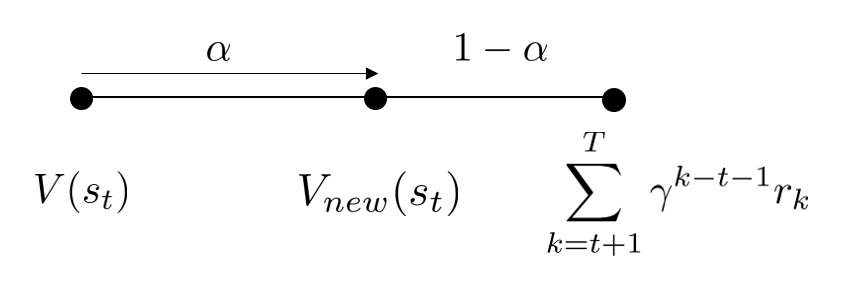
\includegraphics[width=7cm]{monte.png}
    \caption{モンテカルロ法の幾何的な意味}
    \label{fig:monte}
\end{figure}
\newpage
\subsection{TD法}
\begin{algorithm}[TD(0)法]
    \begin{equation}
        V(s_t)\leftarrow V(s_t)+\alpha(r_{t+1}+\gamma V(s_{t+1})-V(s_t))
    \end{equation}
\end{algorithm}
ベルマン方程式の解$V(s_t)=r_{t+1}+\gamma V(s_{t+1})$を用いてエピソード終了の終了を待たずに更新を行う.そのためモンテカルロ法のように修正前の行動が延々と続けられることはない.しかし,見積もりによる更新が行われるため正確性に欠けるというデメリットがある.\\
$V(s_{t+1})$についてベルマン方程式を用いて展開すると,
\begin{equation}
    V(s_t)\leftarrow V(s_t)+\alpha(r_{t+1}+\gamma r_{t+2}+\gamma^2 V(s_{t+2})-V(s_t))
\end{equation}
が成り立つ.これを2期のMulti-step Learnigという.同様にベルマン方程式を用いることで$k$期$(2\leq k)$のMulti-step Learnigを考えることができ,$k\to \infty$とするとモンテカルロ法と一致することが示される.

\subsection{TD($\lambda$)法}
前節において$k$を固定するTD法を考えたが,複数のstepを組み合わせる手法も考えられる.$k$ step先の価値を$G_t^{(k)}$とする.つまり,
\begin{align*}
    &G_t^{(1)}=r_{t+1}+\gamma V(s_{t+1})\\
    &G_t^{(2)}=r_{t+1}+\gamma r_{t+2}+\gamma^2 V(s_{t+2})\\
    &\ \ \ \  \ \ \ \vdots\\
    &G_t^{(T-t)}=r_{t+1}+\gamma r_{t+2}+\cdots+\gamma^{T-t} r_{_T}
\end{align*}
とする.
これらに関して加重平均を考える.具体的には$0\leq\lambda\leq 1$として,
\begin{equation}
    G_t^{(1)}:G_t^{(2)}:\ldots:G_t^{(T-t)}=1:\lambda:\ldots:\lambda^{T-t-1}
\end{equation}
とする.$\displaystyle \sum_{n=0}^{T-t-1}\lambda^n=1$となるように定数倍を注意すると,
\begin{equation}
    G_t^{\lambda}=(1-\lambda)\sum_{n=1}^{T-t-1}\lambda^{n-1}G_t^{n}+\lambda^{T-t-1}G_t^{(T-t)}
\end{equation}
が導出される.
これは$\lambda$を大きくするにつれ長い経験をより重視することを意味する.特に$\lambda=1$のとき,モンテカルロ法と一致する.
逆に$\lambda=0$の時はTD(0)法と一致する.\\
$\lambda$の値を調整することで長いstepを重視するか短いstepを重視するか調整できるため,TD($\lambda$)法はモンテカルロ法とTD法の折衷案として用いられる.
\section{まとめ}
方策決定の手法と更新アルゴリズムを見てきた.これらと環境を実装することで独自の強化学習を構築することができる.


\chapter{巡回セールスマン問題}
巡回セールスマン問題とは,以下のような問題である.\\ \\
頂点数$N$の重み付き有向グラフの隣接行列$D$が与えられる.\ 頂点$s$から頂点$t$への道の集合の中で重みの総和が最小の道を求める
\section{道の全列挙}
始点$s$と終点$t$を除く$1$から$n$の順列を全列挙し,それらのpathにおいて辺の重みの総和の最小値が解になる.
このとき順列の個数は,$(N-2)!$なので,巡回セールスマン問題を時間計算量$O((N-1)!)$で求めることができた.

\section{集合に対する動的計画法}
$S$を既に訪れた頂点集合,現在頂点$v$にいるとする.
$$dp(S,v)=(vに来るまでにかかる距離の総和の最小値)$$
このとき,以下の漸化式が成立.
\begin{eqnarray}
    \begin{cases}
        & dp(\{s\},s)=0\\ \\
        & \displaystyle dp(S,v)=\min_{u \notin S}(dp(S\setminus\{u\},u)+D_{u,v})
    \end{cases}
\end{eqnarray}
$X=\{1,2\ldots ,n\}$としたとき,巡回セールスマン問題の解は$dp(X,t)$である.\\
よって時間計算量$O(2^NN^2)$で解くことができた.
\section{ヒューリスティックな解法}
集合に対する動的計画法を用いた解法は$N$が大きくなるにつれて指数的に時間計算量が大きくなる.そのため頂点数が大きいグラフの巡回セールスマン問題は現実的な時間で計算結果を出すことができない.
例えば山登り法や焼きなまし法,遺伝的アルゴリズムを用いることにより多項式時間で近似解を求めることができる.

\chapter{問題設定}
\section{具体的な問題設定}
京都府の観光地(25地点)に関するデータを用いて以下の条件の下で総合魅力度の総和を最大化する.
\begin{enumerate}
    \item 始点は京都駅,終点は祇園のpathである.
    \item 合計所要時間は300分である.
    \item 任意の頂点(観光地)の滞在時間は30分である.
    \item 任意の頂点$i,j$ついて$i$から$j$への移動は$D_{i,j}$分かかる.
    \item 任意の頂点$i$には総合魅力度$C_i$が設定されていて,頂点$i$を訪れると報酬$C_i$を得る
    \item 任意の頂点$i$について$D_i$の値の中から小さい順に5つの頂点にのみ辺を結ぶ.
    \item 例外として京都タワーの入次数は1で京都駅からのみ行くことができる.
    \item 行列$D$の成分は整数である.
\end{enumerate}
条件の7は京都駅から京都タワーへは徒歩2分で行けるため外れ値として設定した.
\section{抽象化}
自己閉路を持たない頂点数$N$の重み付き有向グラフ$G$を考える.$G$の任意の頂点$i$には報酬$C_i$が設定されている.
$s$から$t$へのpathを$s=p_0\to p_1 \ldots p_{m-1}\to p_m=t$としたとき,
\begin{equation}
    \sum_{i=0}^{m-1} D_{p_i,p_{i+1}}\leq T
\end{equation}
のもとで
\begin{equation}
    \sum_{i=0}^{m} C_{p_i}
\end{equation}
を最大化する.
\section{厳密解}
巡回セールスマン問題と同様の手法で求めることができる.
\subsection{解法1}
始点$s$,終点$t$の全ての列の中で,条件を満たすものの中で報酬の総和が最大のものを出力する.\\
これは$\displaystyle O\left(\sum_{k=1}^{N-1}k!\right)$で達成できる.
\subsection{解法2}
$S$を既に訪れた頂点集合,現在頂点$v$にいて,時刻$t$とする.
$$dp(S,v,t)=(vに来るまでに得た報酬の最大値)$$
このとき,$0\leq t\leq T$に関して以下の漸化式が成立.
\begin{eqnarray}
    \begin{cases}
        & \displaystyle dp(S,v,t)=\max_{u \notin S}(dp(S\setminus\{u\},u,t-D_{u,v})+C_v)\ \ \ \  (t-D_{u,v}\geq0)\\
        & dp(S,v,t)=0 \ \ \ \ ({\rm otherwise})
    \end{cases} 
\end{eqnarray}
時間計算量は$O(2^NN^2T)$である.

\chapter{手法}
強化学習を用いて多項式時間で5章の問題の近似解を求める.
\section{手法の選択}
時間制限が$300$分で$1$つの観光地に対して$30$分滞在する.そのため,pathの長さは高々$9$と短くなるので,モンテカルロ法の「エピソード終了時まで修正ができないので最適でないと途中で分かっていてもエピソード終了まで続けないといけない」はデメリットになり得ない.そのためモンテカルロ法を使用する.また行動は$\varepsilon-$greedy法に基づいて行う.
\section{環境の設定}
\subsection{状態空間}
一度訪れた頂点は再度訪問することができないため,この環境はマルコフ性を持つことが難しい.実際には既に訪れた頂点集合$S$,現在いる頂点$v$,現在時刻$t$が必要である.pathの長さが高々$9$である上に$D_{i,j}$の値も大きいため,$S,v,t$の全ての情報を持つ空間に対して実際に観測できる空間は非常に少ない.そこで,状態をハッシュ化して状態の情報量を落としながら疑似的なマルコフ性を持つ環境を作ることを考える.以下の3つが考えられる.
\begin{itemize}
  \item $S$と$t$の情報を落とす.
  \item $S$の情報を落とす.
  \item $t$の情報を落とす.
\end{itemize}
例えば$S$と$t$の情報を落としたとき,どのような経路を辿ったとしても頂点$v$では全く同じ行動を返すagentが完成する.$S$と$t$の情報を落としたときと,$t$の情報を落としたとき,頂点$v$に辿り着くまでの経路の長さを$k$とするとハッシュのkeyは$(k-2)!$回以上の衝突が起きることになる.それに対し,$D$は多様な値を取るため,$S$の情報を落とした時は終点が$v$であるような辺の列$P,P'\ (P\not=P')$に対して,
\begin{equation}
    \sum_{e \in P} e= \sum_{e \in P'} e
\end{equation}
となる場合は稀であると考えらえる.
そのためagentには現在いる頂点$v$と現在時刻$t$の2つの状態を渡す.

\subsection{行動空間}
実装を簡単にするため任意の頂点に行動できるとする.ただし,辺が存在しない場合は距離を$\infty$とする.
\subsection{即時報酬}
以下のような報酬を返す.
\begin{itemize}
  \item 時間制限を超えると$-100$の報酬を得る.
  \item すでに訪れた頂点を選択すると$-1$の報酬を得る.
  \item ゴールに辿り着くと$0$の報酬を得る.
  \item それ以外の場合は訪れた頂点を$v$とすると,$100C_v$の報酬を得る.
\end{itemize}
\subsection{終了条件}
時間制限を超えた時とゴールに辿り着いたときに限りエピソードを終了する.
\section{その他}
\subsection{並列化}
強化学習は局所最適解に陥ることが多いため複数回実行する必要がある.そのため学習はPythonの非同期並列処理を用いて合計$96$回の学習を行う.\\ 
($96$回は学習に用いた計算機のCPUのスレッド数が$16$で$96=16*6$に起因する.)
\subsection{出力部分}
学習は合計所要時間が$300$分以下になるように行われるが,それ以下の最適化は行われない.そこで,学習で得られた経路のグラフを部分グラフとして巡回セールスマン問題を解く.これによって最短経路長となるグラフを新たに再構築する.またグラフの頂点数が高々$9$であるため,集合に対する動的計画法を用いる.
\section{まとめ}
学習モデルをフローチャートにしてまとめる.
\begin{figure}[h]
    \centering
    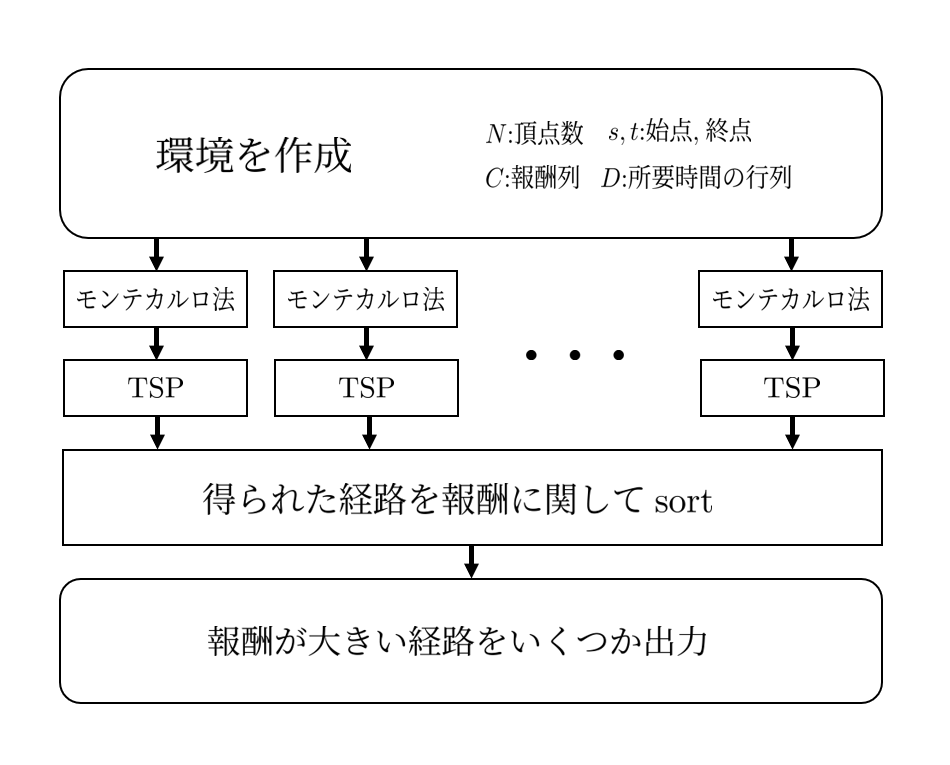
\includegraphics[width=9cm]{model.png}
    \caption{フローチャート}
    \label{fig:model}
\end{figure}

\chapter{結果・考察}
\section{結果}
付録Aの使用コードの結果を記載する.エピソードの反復回数は$10^7$回で,$96$回の独立な学習を行った.まずは全体図である.
\begin{figure}[h]
    \centering
    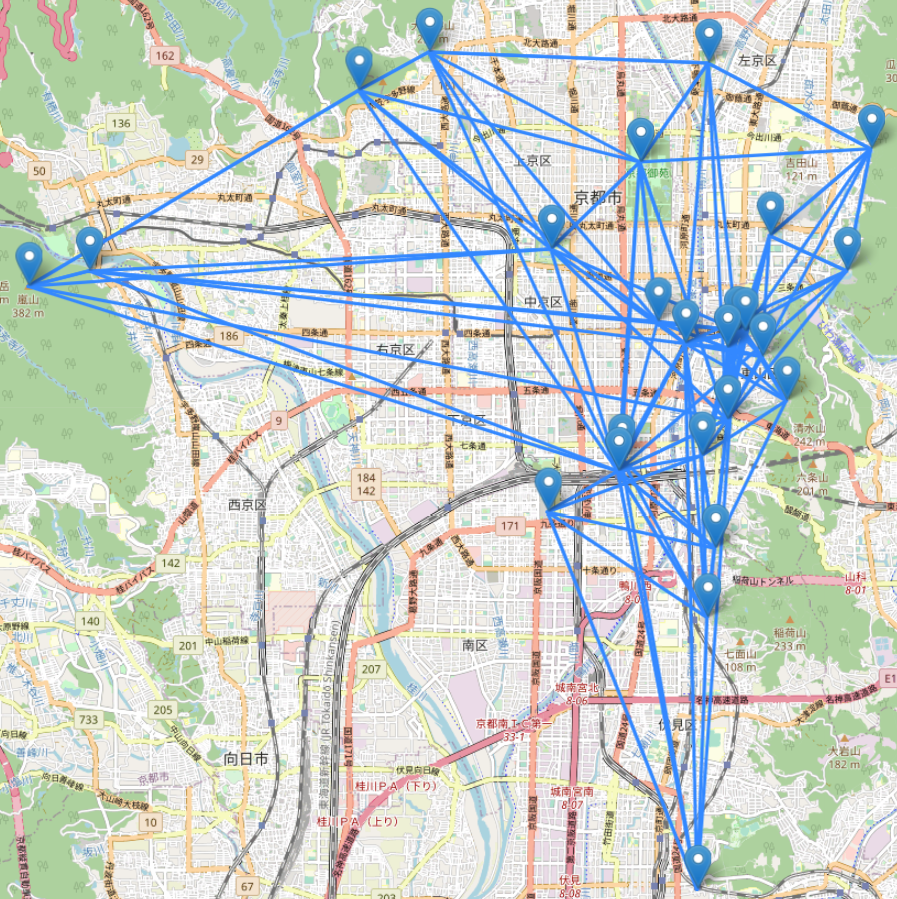
\includegraphics[width=9cm]{png/round.png}
    \caption{全体図}
    \label{fig:round}
\end{figure}
\newpage
各地域の報酬列に対しての結果である.左から1位,3位,5位の順に載せている.
\begin{figure}[htbp]
    \begin{minipage}{0.49\hsize}
        \begin{center}
            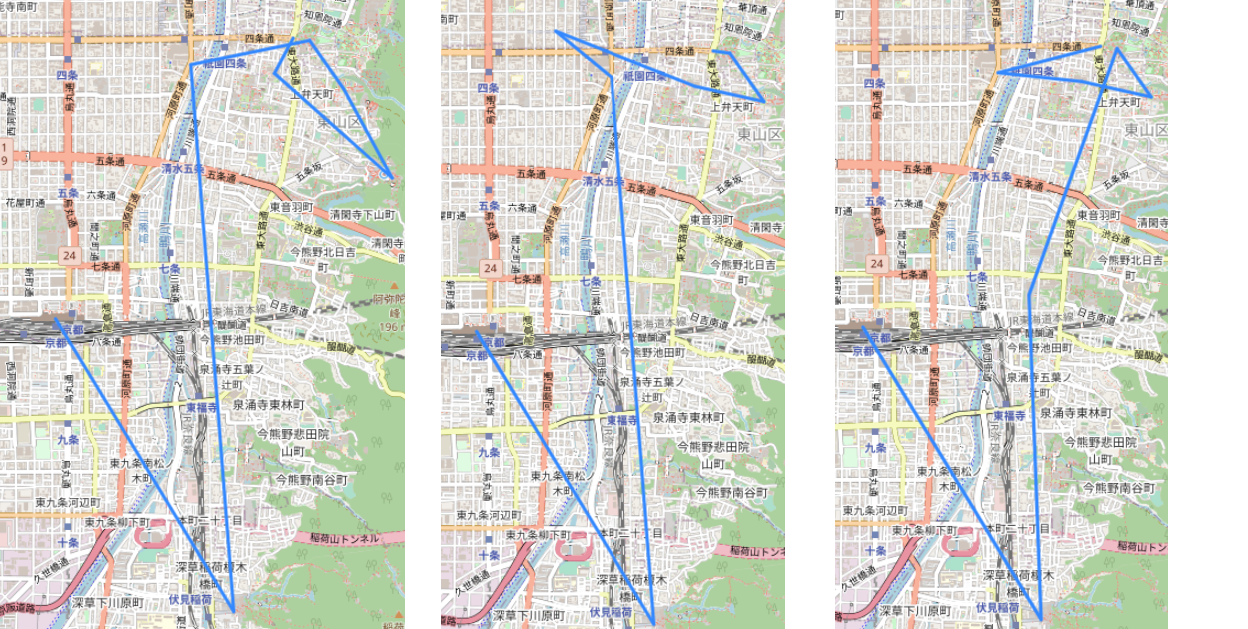
\includegraphics[width=61mm]{png/china.png}
        \end{center}
        \caption{中国}
        \label{fig:china}
    \end{minipage}
    \begin{minipage}{0.49\hsize}
        \begin{center}
            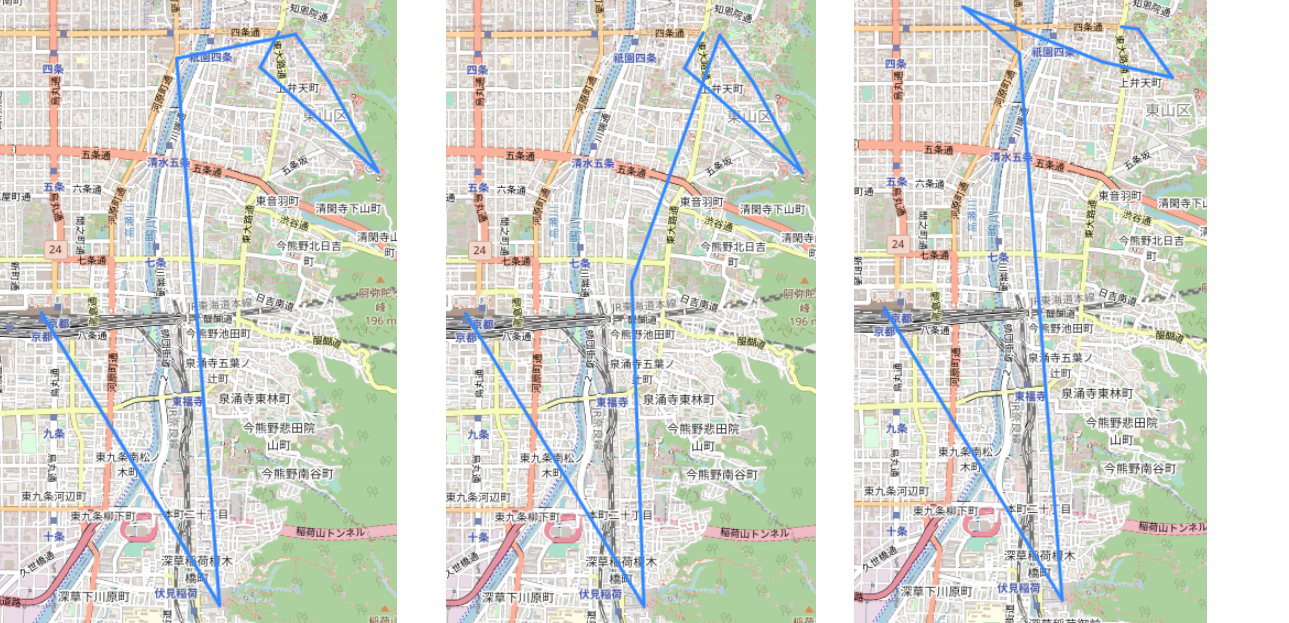
\includegraphics[width=61mm]{png/hokubei.png}
        \end{center}
        \caption{北米}
        \label{fig:hokubei}
    \end{minipage}
\end{figure}
\begin{figure}[htbp]
    \begin{minipage}{0.49\hsize}
        \begin{center}
            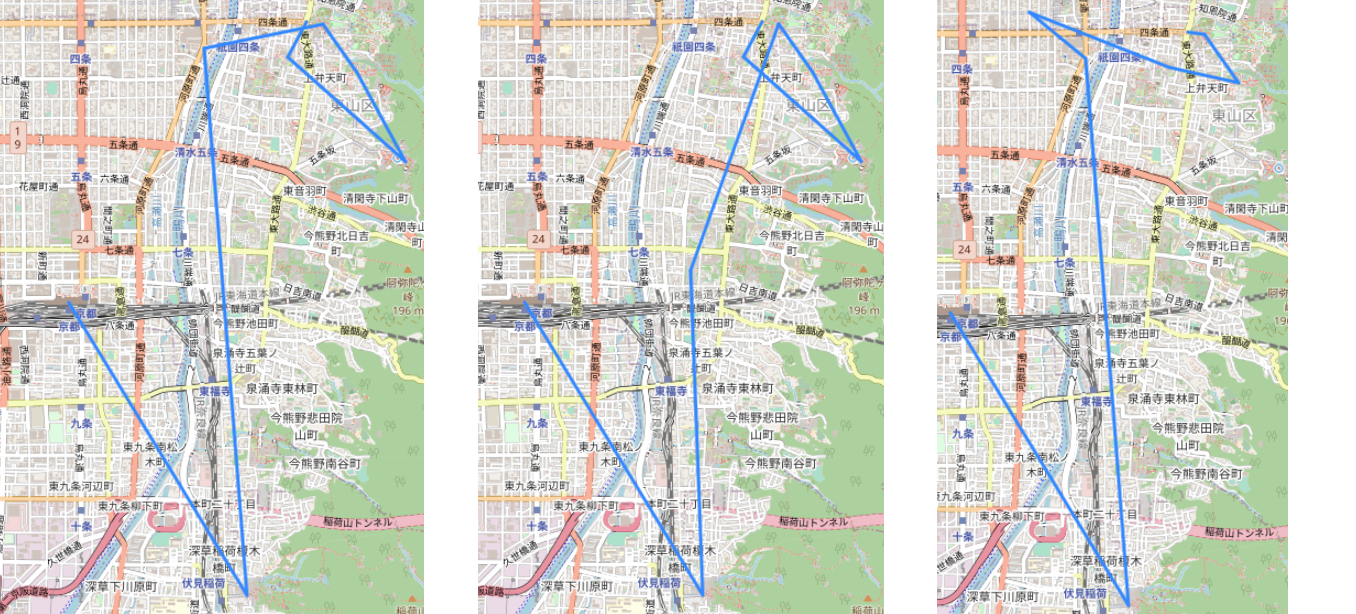
\includegraphics[width=61mm]{png/honkon.png}
        \end{center}
        \caption{香港}
        \label{fig:honkon}
    \end{minipage}
    \begin{minipage}{0.49\hsize}
        \begin{center}
            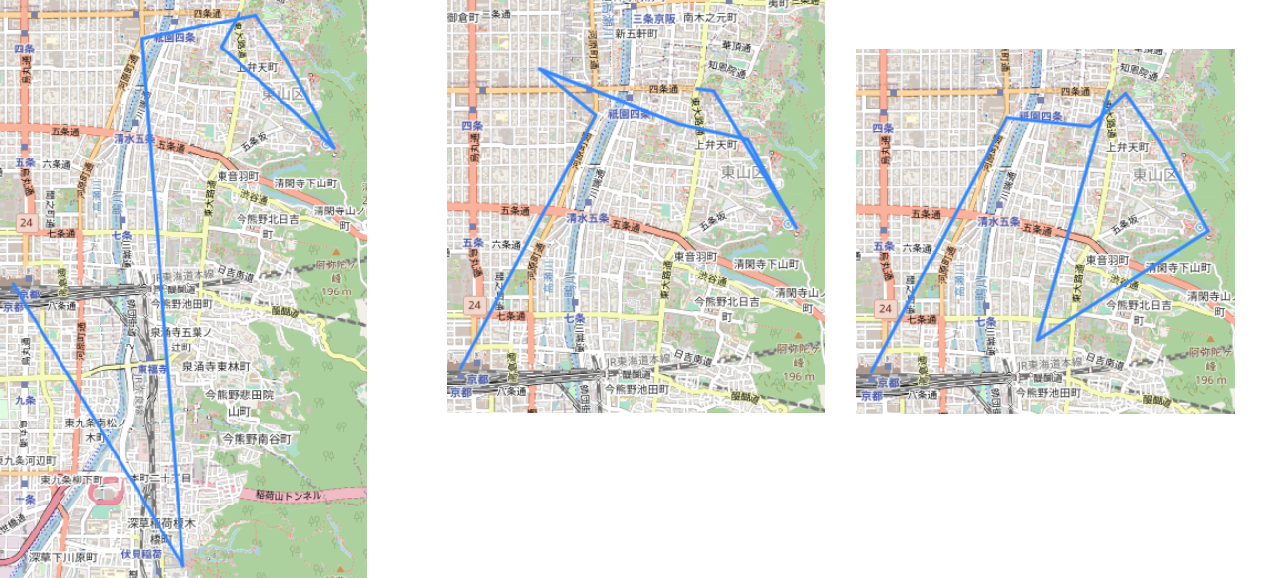
\includegraphics[width=61mm]{png/korea.png}
        \end{center}
        \caption{韓国}
        \label{fig:korea}
    \end{minipage}
\end{figure}

\begin{figure}[htbp]
    \begin{minipage}{0.49\hsize}
        \begin{center}
            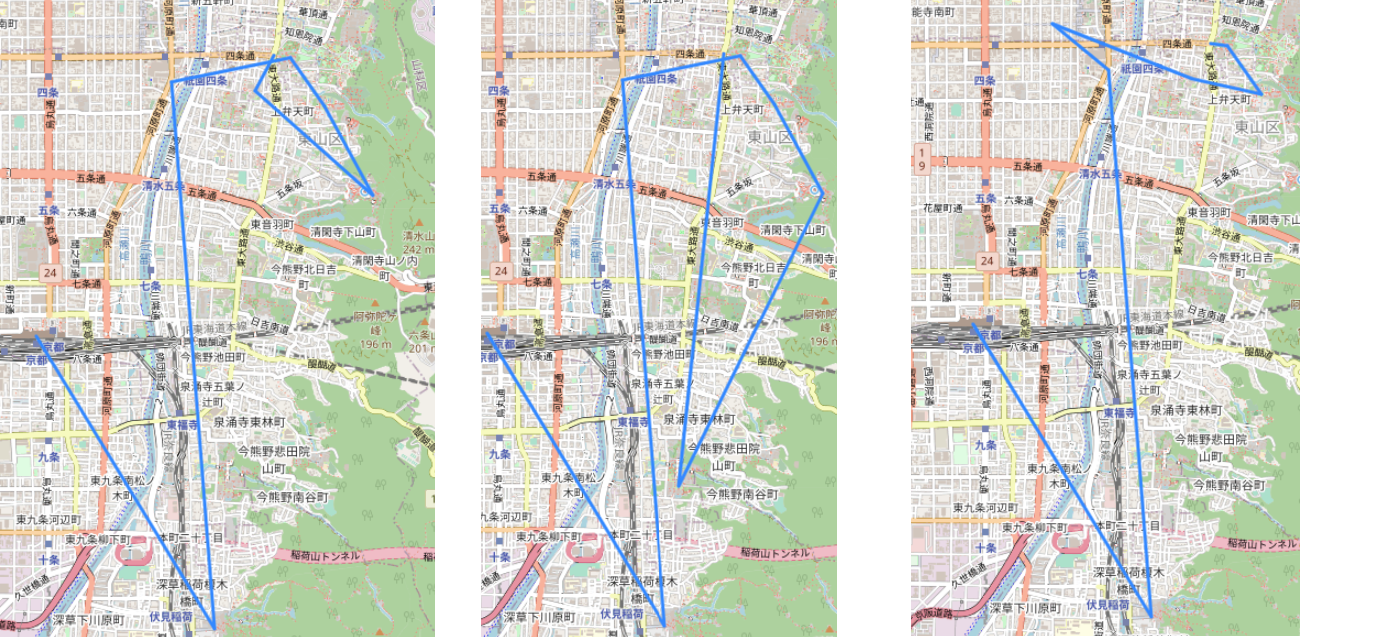
\includegraphics[width=61mm]{png/oseania.png}
        \end{center}
        \caption{オセアニア}
        \label{fig:oseania}
    \end{minipage}
    \begin{minipage}{0.49\hsize}
        \begin{center}
            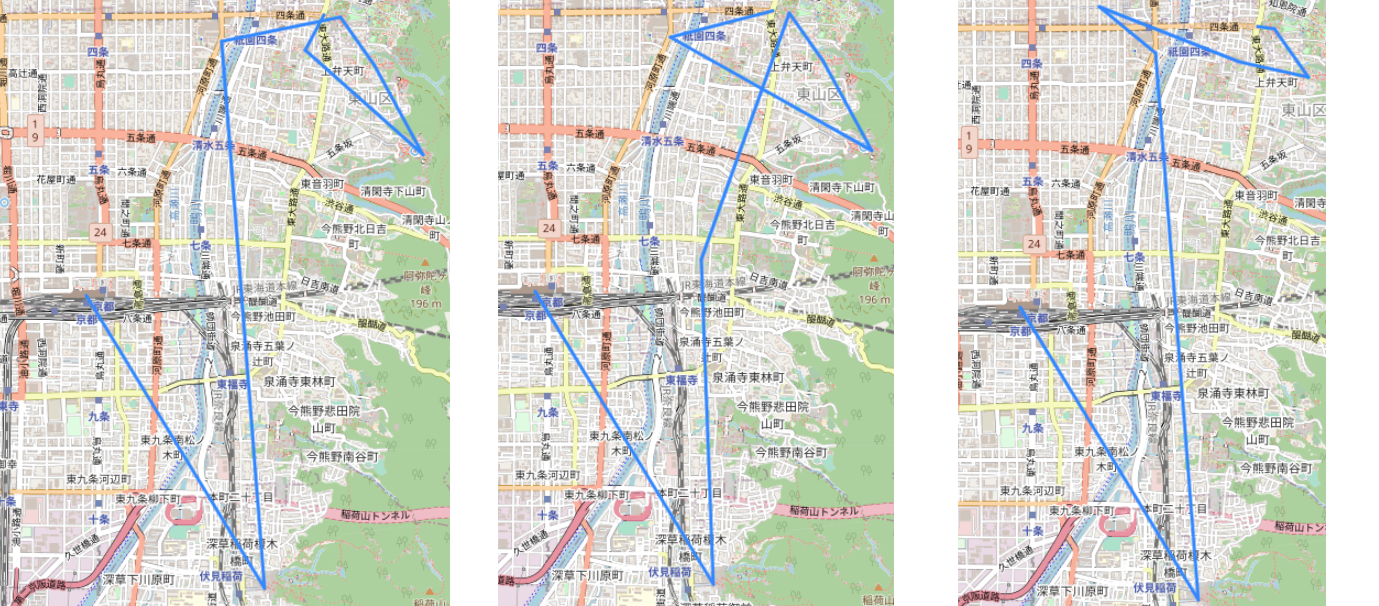
\includegraphics[width=61mm]{png/oushuu.png}
        \end{center}
        \caption{欧州}
        \label{fig:oushuu}
    \end{minipage}
\end{figure}
\newpage
\begin{figure}[htbp]
    \begin{minipage}{0.49\hsize}
        \begin{center}
            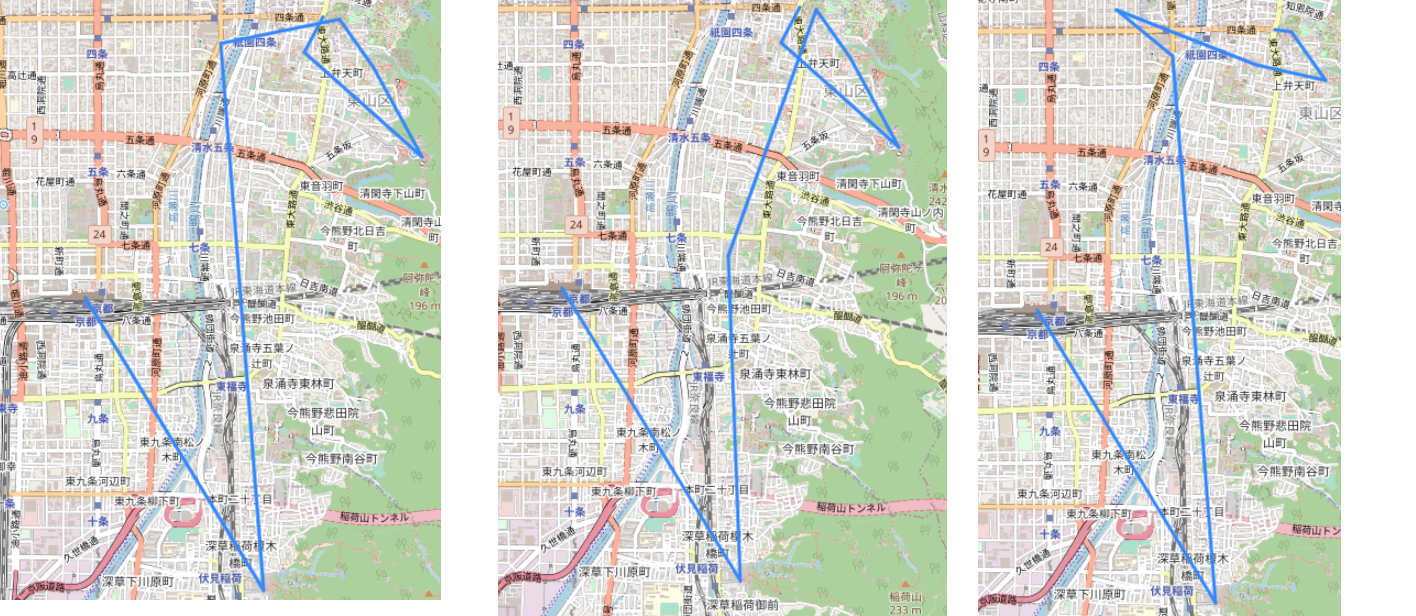
\includegraphics[width=61mm]{png/taiwan.png}
        \end{center}
        \caption{台湾}
        \label{fig:taiwan}
    \end{minipage}
    \begin{minipage}{0.49\hsize}
        \begin{center}
            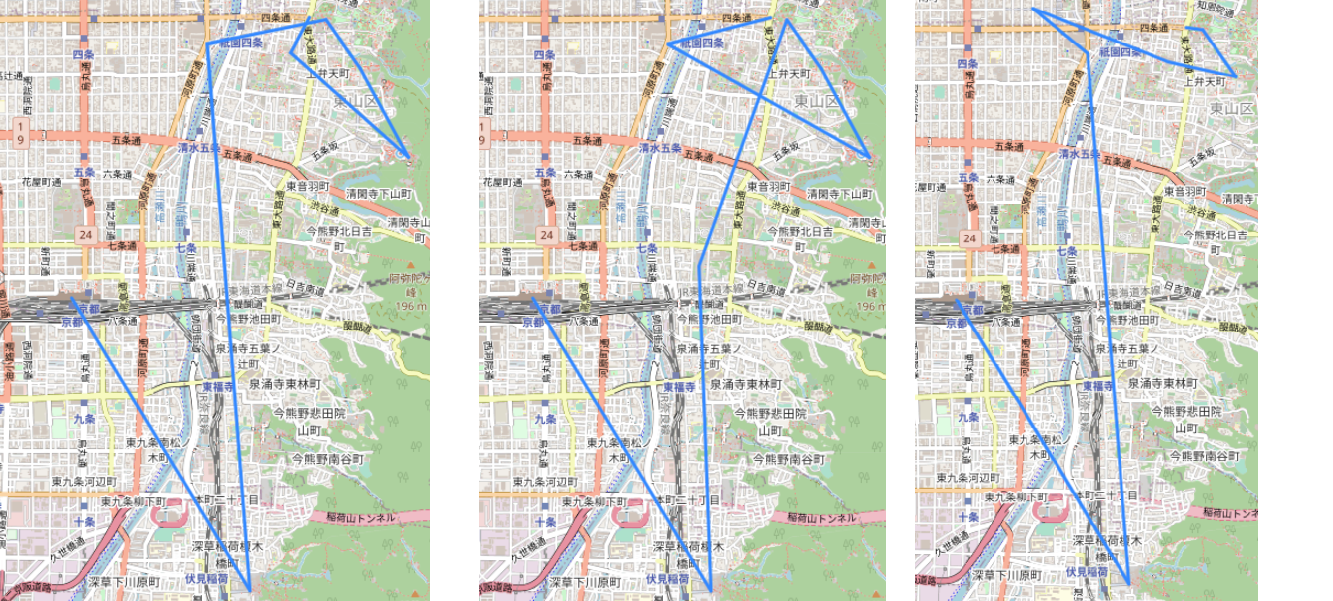
\includegraphics[width=61mm]{png/tounanazia.png}
        \end{center}
        \caption{東南アジア}
        \label{fig:tounanazia}
    \end{minipage}
\end{figure}
\section{考察}
各国に対して1位,3位,5位のほとんどのagentは報酬が高い伏見稲荷や清水寺を訪れ,報酬が高い地点の付近を周遊する直感に近い結果となった.これは報酬列の与え方や実装が適切であることを示している.下に報酬列を$0.1$倍した他は同じ条件下での中国の1位,3位(5位は現れなかった)を載せる.各国の報酬列が似たような値を取るため各国の1位が同じルートを示した.これはうまく学習できていることを示している.しかし,これは各国同士の差別化ができていない
\begin{figure}
    \centering
    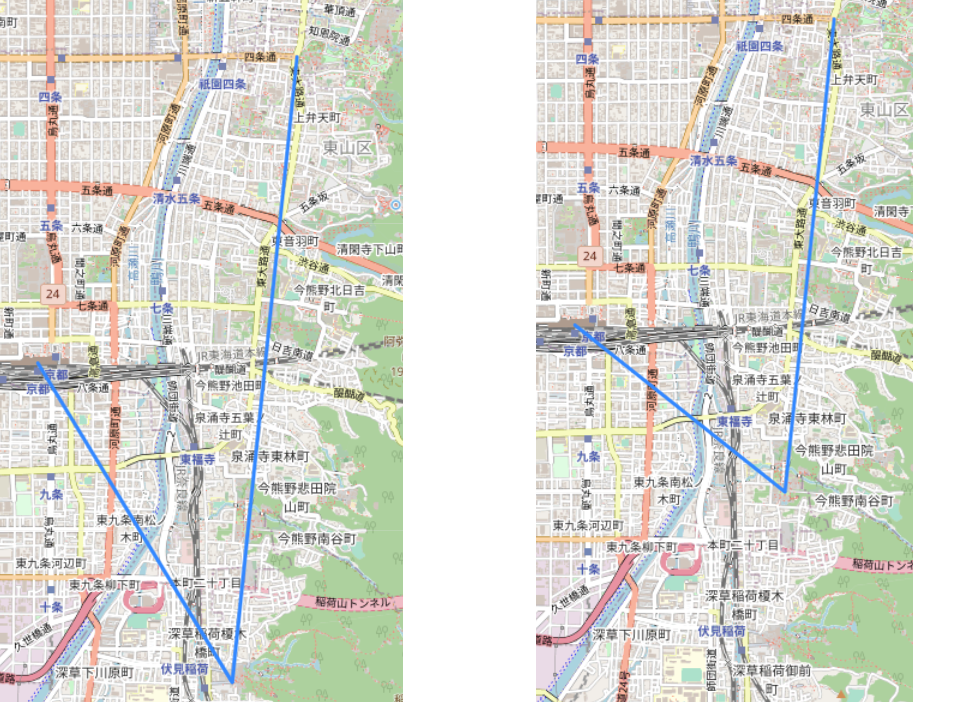
\includegraphics[width=9cm]{png/01.png}
    \caption{報酬列を0.1倍したもの(うまくいかなかった例)}
    \label{fig:01}
\end{figure}


\chapter{追加実験}
各国に対してあまり結果は変わらないことがわかった.そこで,さらに以下のような追加実験を行った.
\section{問題設定}
5章のルールをほとんどそのまま使用する.追加で以下のようなルールを課す.
\begin{itemize}
    \item 始点,終点以外にいくつか必ず通らないといけない頂点が指定される.
    \item 指定された頂点は任意の頂点に隣接している.
\end{itemize}
\section{手法}
6章の手法をほとんどそのまま使用する.ただし,必ず通らないといけない頂点の報酬を元の報酬列の最大値の2倍に変更する.各国に対してあまり結果は変わらないことが予想されるため中国にのみ実験する.また,通らないといけない頂点は嵐山とする.
\section{結果・考察}
時間いっぱいまで使って嵐山を通るルートを示した.agentは貪欲に学習するため,初手に嵐山に行くルートを過剰に評価するが,1位は初手に嵐山に行かないルートを選択したため学習は成功したと言っていいだろう.(出力結果は巡回セールスマン問題を解いているが,1位の頂点集合で初手以外に祇園に行くと時間に間に合わない.)
\begin{figure}
    \centering
    \includegraphics[width=13cm]{png/all.png}
    \caption{左上1位,右上3位,左下5位,右下7位}
    \label{fig:all}
\end{figure}



\chapter{最後に}
強化学習による最適観光ルート推定を行うモデルの構築を行った.ルート推定はうまくいっていると言って良いだろう.しかし実際にこのモデルを使用するにあたって学習に1.5時間から2時間かかるという問題点がある.そこで以下では高速化手法を2つ紹介する.
\section{高速な言語を使う}
付録に載せている通り,学習にはPython3を使用した.外部ライブラリはほとんど使用していないそのためC++やRustのような高速な言語の移植が比較的容易である.これにより30~100倍程度の高速化が見込まれる.そのほかにもCythonやPyPyを使うことによってほとんどそのままのコードである程度高速に動かせることができる.
\section{グラフの構造を変える}
実装を容易にするため完全グラフを用いた.実際は隣接していない頂点は距離$\infty$で表現した.完全グラフにするのではなく,行動空間を制限することにより同じ結果を出すための学習回数を$1/4$倍で抑えることが見込まれる.
\\ \\
1と2を用いて120~400倍の高速化が見込まれて,学習時間を1分以下に抑えることができると予想できる.


\chapter*{謝辞}
本研究に際して、様々なご指導を頂きました津田先生,大
学院生の先輩方に深謝いたします。また本研究の根幹にあたるアルゴリズムの学習の機会を与えてくれたAtCoder株式会社様には深くお礼申し上げます。


\appendix

\chapter{使用したコード}
コードの依存関係は以下の通りである.
\begin{figure}[htbp]
    \centering
    
\includegraphics[width=13cm]{izon.png}
    \caption{コードの依存関係}
    \label{fig:izon}
\end{figure}
\newpage
get\_data.py
\begin{lstlisting}[caption=, label=, language=Python]
import xlrd
import pprint
import os
os.chdir(os.path.dirname(os.path.abspath(__file__)))

import numpy as np
from math import sqrt, pi, cos, sin, acos


def distance(From, To):
    """東経と北緯が与えられて距離を返す."""
    x0, y0 = From
    x1, y1 = To
    x0 *= pi / 180
    x1 *= pi / 180
    y = pi * (y1 - y0) / 180
    return 6378137 * acos(sin(x0) * sin(x1) + cos(x0) * cos(x1) * cos(y))


def get_list_2d(sheet, start_row, end_row, start_col, end_col):
    """[start_row, end_row)*[start_col, end_col)の行列を取得"""
    return [list(map(int, sheet.row_values(row, start_col, end_col)))
            for row in range(start_row, end_row)]


def get_time(*go, stay=0, edge_limit=6):
    """距離行列(time)を返す"""
    """
     stay:滞在時間
     edge_limit:自身を含む辺をつなぐ数
    """
    wb = xlrd.open_workbook('data/time.xlsx')
    sheet = wb.sheet_by_name('data_only')
    d = np.array(get_list_2d(sheet, 0, 25, 0, 25))
    d += stay
    spots = get_spots()
    go = {spots.index(spot) for spot in go}
    compress = np.argsort(np.argsort(d))
    for i in range(25):
        if i != 12:
            d[i][11] = 100_000_000

    for i in range(25):
        for j in range(25):
            if compress[i][j] > edge_limit and i not in go and j not in go:
                d[i][j] = 100_000_000
    return d


def get_happiness(country, *go):
    """幸福度を返す"""
    """warning:各幸福度が100以上になってはならない"""
    wb = xlrd.open_workbook('data/AHP.xlsx')
    sheet = wb.sheet_by_name(country)
    col = ord("K") - ord("A")
    spots = get_spots()
    happiness = np.array([sheet.cell_value(row, col) for row in range(3, 28)]) * 100
    s = 2 * happiness.max()
    for spot in go:
        happiness[spots.index(spot)] = s
    return np.array(happiness)


def get_spots():
    """都市を返す"""
    wb = xlrd.open_workbook('data/time.xlsx')
    sheet = wb.sheet_by_name('name_and_data')
    spots = [sheet.cell_value(row, 0) for row in range(6, 31)]
    return spots


def get_distance():
    """緯度, 経度情報から距離行列を返す"""
    pos = \
        {'清水寺': (34.994856, 135.785046),
         '二条城': (35.01423, 135.748218),
         '伏見稲荷': (34.96714, 135.772672),
         '金閣寺': (35.03937, 135.729243),
         'ギオンコーナー': (35.001551, 135.775822),
         '嵐山': (35.009449, 135.666773),
         '祇園': (35.003782, 135.777245),
         '八坂神社': (35.003656, 135.778553),
         '京都御所': (35.025414, 135.762125),
         '銀閣寺': (35.027021, 135.798206),
         '錦市場': (35.005008, 135.764902),
         '京都タワー': (34.987531, 135.759324),
         '京都駅': (34.985849, 135.758767),
         '龍安寺': (35.034494, 135.718263),
         '伏見': (34.932416, 135.771056),
         '東寺': (34.980598, 135.747786),
         '高台寺': (35.00051, 135.781218),
         '南禅寺': (35.011414, 135.794484),
         '東福寺': (34.976064, 135.773777),
         '平安神宮': (35.015982, 135.782426),
         '嵐山モンキーパーク': (35.011408, 135.676206),
         '東山': (34.992396, 135.775797),
         '河原町': (35.002111, 135.769279),
         '三十三間堂': (34.987885, 135.771713),
         '下鴨神社': (35.038037, 135.772773)}
    pos = list(pos.values())
    dist = np.zeros((25, 25))
    for i, e in enumerate(pos):
        for j, f in enumerate(pos):
            dist[i, j] = distance(e, f)
    return dist
\end{lstlisting}
Kyoto\_env\_ontime.\_\_init\_\_.py
\begin{lstlisting}[caption=, label=, language=Python]
from gym.envs.registration import register

register(
    id='Kyoto_ontime-v0',
    entry_point='Kyoto_env_ontime.env:Kyoto_ontime'
)

\end{lstlisting}
Kyoto\_env\_ontime.env.py
\begin{lstlisting}[caption=, label=, language=Python]
import sys
import gym
import numpy as np
import gym.spaces


class Kyoto_ontime(gym.Env):
    def __init__(
            self, n: "頂点数",
            start: "始点",
            goal: "終点",
            happiness: "幸福度のリスト",
            time_limit: "時間制限",
            distance: "隣接行列",
            d: "時間"):
        super().__init__()
        self.n = n
        self.start = start
        self.goal = goal
        self.happiness = happiness
        self.time_limit = time_limit
        self.distance = distance
        self.d = d
        self.observation_space = gym.spaces.Box(low=0, high=n, shape=(n,))
        self.action_space = gym.spaces.Discrete(n)
        self.reward_range = [-1., 100.]
        self.reset()

    def reset(self):
        # 諸々の変数を初期化する
        self.pos = self.start
        self.done = False
        self.steps = 0
        self.time = 0
        self.use = [0] * self.n
        self.use[self.start] = 1
        # if self.start == 12:
        #     self.use[11] = 1
        #     self.time += 30
        return self._observe()

    def _render(self):
        pass

    def _close(self):
        pass

    def _seed(self, seed=None):
        pass

    def step(self, action):
        # 1ステップ進める処理を記述。戻り値は observation, reward, done(ゲーム終了したか), info(追加の情報の辞書)
        next_pos = action

        if self._is_movable(next_pos):
            self.time += self.d[self.pos][next_pos]
            self.use[next_pos] = 1
            self.pos = next_pos
            moved = True
        else:
            moved = False

        observation = self._observe()

        reward = self._get_reward(self.pos, moved)
        self.done = self._is_done()
        return observation, reward, self.done, {}

    def _is_movable(self, next_pos):
        """合法手か否か. use[pos]なら既に行った場所なので非合法"""
        return 1 - self.use[next_pos]

    def _get_reward(self, pos, moved):
        """報酬を返す. 再考の余地あり"""
        if self._is_game_over():
            return -100
        if not moved:
            return -1
        if self.goal == pos:
            return 0
        return self.happiness[pos]

    def _observe(self):
        return (self.pos, self.time)

    def _is_done(self):
        """時間切れかゴールにたどり着くとdone"""
        return self.pos == self.goal or self.time_limit < self.time

    def _is_game_over(self):
        return self.time_limit < self.time
\end{lstlisting}
el\_agent.py
\begin{lstlisting}[caption=, label=, language=Python]
import numpy as np
import matplotlib.pyplot as plt
from collections import defaultdict


class ELAgent():

    def __init__(self, epsilon, env):

        self.Q = {}
        self.epsilon = epsilon
        self.reward_log = []

    def policy(self, s, actions):
        """epsilonでランダム, それ以外でargmax"""
        if np.random.rand() < self.epsilon:
            return np.random.randint(len(actions))
        else:
            if s in self.Q and sum(self.Q[s]) != 0:
                return np.argmax(self.Q[s])
            else:
                return np.random.randint(len(actions))

    def init_log(self):
        self.reward_log = []

    def log(self, reward):
        self.reward_log.append(reward)

    def show_reward_log(self, interval=50, episode=-1):
        """intervalおきのsummaryを表示"""
        if episode > 0:
            rewards = self.reward_log[-interval:]
            mean = np.round(np.mean(rewards), 3)
            std = np.round(np.std(rewards), 3)
            print("At Episode {} average reward is {} (+/-{}).".format(
                episode, mean, std))

        else:
            indices = list(range(0, len(self.reward_log), interval))
            means = []
            stds = []
            for i in indices:
                rewards = self.reward_log[i:i + interval]
                means.append(np.mean(rewards))
                stds.append(np.std(rewards))
            means = np.array(means)
            stds = np.array(stds)
            plt.figure()
            plt.title("Reward History")
            plt.grid()
            plt.fill_between(indices, means - stds, means + stds,
                             alpha=0.1, color="g")
            plt.plot(indices, means, "o-", color="g",
                     label="Rewards for each {} episode".format(interval))
            plt.legend(loc="best")
            plt.show()

\end{lstlisting}
monte\_carlo\_ontime.py
\begin{lstlisting}[caption=, label=, language=Python]
import math
from collections import defaultdict
from el_agent import ELAgent
import numpy as np


class MonteCarloAgent(ELAgent):

    def __init__(self, env, epsilon=0.1):
        super().__init__(epsilon, env)

    def learn(self, env, episode_count=1000, gamma=0.9,
              render=False, report_interval=50, show_log=True):
        self.init_log()
        actions = list(range(env.action_space.n))
        if not self.Q:
            self.Q = defaultdict(lambda: [0] * len(actions))
        N = defaultdict(lambda: [0] * len(actions))

        for e in range(episode_count):
            s = env.reset()  # 初期化して環境を取得
            done = False
            # Play until the end of episode.
            experience = []
            sum_reward = 0
            while not done:
                if render:
                    env.render()
                a = self.policy(s, actions)
                n_state, reward, done, _ = env.step(a)
                experience.append({"state": s, "action": a, "reward": reward})
                s = n_state
                sum_reward += reward
            else:
                self.log(sum_reward)

            # Evaluate each state, action.
            for i, x in enumerate(experience):
                s, a = x["state"], x["action"]

                # Calculate discounted future reward of s.
                G, t = 0, 0
                for j in range(i, len(experience)):
                    G += math.pow(gamma, t) * experience[j]["reward"]
                    t += 1

                N[s][a] += 1  # count of s, a pair
                alpha = 1 / N[s][a]
                # 更新式
                self.Q[s][a] += alpha * (G - self.Q[s][a])
            if show_log and e != 0 and e % report_interval == 0:
                self.show_reward_log(episode=e, interval=report_interval)

\end{lstlisting}
train\_ontime.py
\begin{lstlisting}[caption=, label=, language=Python]
import gym
import Kyoto_env_ontime
from get_data import get_time, get_happiness, get_distance
import numpy as np
from monte_carlo_ontime import MonteCarloAgent
from q_learning_ontime import QLearningAgent
from play import play
from collections import defaultdict


def make_env(n=25, start=12, goal=6, country="中国", stay=30):
    """標準は京都駅スタート, 祇園解散"""
    d = get_time(stay=stay)
    happiness = get_happiness(country) * 100
    distance = get_distance()
    time_limit = 300
    env = gym.make("Kyoto_ontime-v0",
                   n=n, start=start, goal=goal,
                   happiness=happiness,
                   time_limit=time_limit,
                   distance=distance,
                   d=d)
    return env


def train(Agent=MonteCarloAgent,
          episode_count=1,
          epsilon=0.1,
          report_interval=1,
          country="中国",
          save=False):
    env = make_env(country=country)
    agent = Agent(epsilon=epsilon, env=env)
    agent.learn(env, episode_count=episode_count, report_interval=report_interval, show_log=False)
    # show_q_value(agent.Q)
    if not save:
        agent.show_reward_log(interval=report_interval)
    else:
        Q = agent.Q
        return dict(Q)
\end{lstlisting}
play.py
\begin{lstlisting}[caption=, label=, language=Python]
import gym
import Kyoto_env_ontime
from get_data import get_spots
import numpy as np


def play(env, Q, show_mode=0):
    """
        show_mode 0: ["京都駅", ..., "祇園"]
                  1: "京都駅 -> .... -> 祇園"
                  2: [12, ..., 6]
    """
    s = env.reset()
    actions = list(range(env.action_space.n))
    done = False
    sum_reward = 0
    reward = 0
    experiece = [env.pos]
    while not done:
        if s not in Q or reward < 0:
            a = np.random.randint(len(actions))
        else:
            a = np.argmax(Q[s])
        n_state, reward, done, _ = env.step(a)
        s = n_state
        experiece.append(s[0])
        sum_reward += reward

    g = get_spots()
    return ((sum_reward, env.time), " -> ".join(map(lambda x: g[x], experiece))) if show_mode == 1 \
        else ((sum_reward, env.time), list(map(lambda x: g[x], experiece))) if show_mode == 0\
        else ((sum_reward, env.time), experiece)

\end{lstlisting}
TSP.py
\begin{lstlisting}[caption=, label=, language=Python]
"""
TSP:
頂点数Nの重み付き有向グラフの距離行列が与えられる.
頂点sからスタートしてk-1個の頂点をちょうど一度ずつめぐってtに行く経路のうち,
重みの総和が最小のものを求める.
ついでに経路復元もする.
"""
from get_data import get_spots


def TSP(n: "頂点数", dist: "距離行列", s: "始点", t: "終点"):
    # dist[i][j] = i->j の距離
    # length:通る頂点の数
    INF = 1_000_000_000

    # dp[S][v] = 集合Sの要素をすべて通って頂点vに行く最短経路長
    # prev[S][v] = 集合Sの要素をすべて通って頂点vに行ったとき, 直前に通った頂点
    dp = [[INF] * n for _ in range(1 << n)]
    prev = [[-1] * n for _ in range(1 << n)]
    dp[0][s] = 0

    for S in range(1 << n):
        for u in range(n):
            if S >> u & 1:
                continue
            for v in range(n):
                if dp[S][u] + dist[u][v] < dp[S + (1 << u)][v]:
                    dp[S + (1 << u)][v] = dp[S][u] + dist[u][v]
                    prev[S + (1 << u)][v] = u

    # 経路復元
    path = [t]
    now, state = t, (1 << n) - 1
    while state > 1:
        state -= 1 << now
        now = prev[state][now]
        path.append(now)

    path.reverse()

    return path


def convert(dist, nodes):
    new_dist = [[0] * len(nodes) for _ in range(len(nodes))]
    new_n = len(nodes)
    for i, e1 in enumerate(nodes):
        for j, e2 in enumerate(nodes):
            new_dist[i][j] = dist[e1][e2]
    tsp = TSP(new_n, new_dist, 0, new_n - 1)
    spots = get_spots()
    return tuple(map(lambda x: spots[nodes[x]], tsp))
\end{lstlisting}
main.py
\begin{lstlisting}[caption=, label=, language=Python]
import gym
import numpy as np
from monte_carlo_ontime import MonteCarloAgent
from q_learning_ontime import QLearningAgent
from play import play
from train_ontime import train, make_env
from multiprocessing import Pool, cpu_count
from time import time
from collections import defaultdict
from TSP import convert
cnt = 0


def _train(a):
    global cnt
    episode_count, epsilon, country = a
    print("start:{}".format(cnt))
    _q = train(Agent=MonteCarloAgent,
               episode_count=episode_count,
               epsilon=epsilon,
               report_interval=1000000,
               country=country,
               save=True)
    print("fininsh:{}".format(cnt))
    cnt += 1

    return (play(make_env(country=country), _q, show_mode=0)[0], _q)


def multi_train(n, episode_count=2000000, country="中国"):
    rand = [0.01, 0.03, 0.05, 0.07, 0.1, 0.15, 0.2, 0.3]
    p = Pool(cpu_count())
    results = p.map(_train, [(episode_count, np.random.choice(rand), country) for i in range(n)])
    p.close()
    return results


def _one_cpu(n):
    rewards = []
    for _ in range(n):
        rewards.append(_train((2000000, 0.1, "中国")))
    print(rewards)


def main_train(country="中国", num_loop=48, train_loop=1000000):
    env = make_env(country=country)
    t = time()
    results = multi_train(num_loop, train_loop, country)
    t = int(time() - t)
    print("{}h {}m {}s".format(t // 3600, (t % 3600) // 60, t % 60))
    results.sort(key=lambda x: x[0], reverse=1)
    # Qs = [v[1] for v in results]
    routes = set()
    unique_results = []
    for score, q in results:
        score, route = play(env, q, show_mode=2)
        route = convert(env.d, tuple(route))

        if route in routes:
            continue
        unique_results.append((score, route))
        routes.add(route)
    unique_results.sort(key=lambda x: x[0], reverse=True)
    # for score, route in unique_results:
    #     print("score:{}, route:{}".format(score, route))
    return unique_results
\end{lstlisting}
viewer.py
\begin{lstlisting}[caption=, label=, language=Python]
import folium


def get_position():
    """緯度, 経度情報"""
    pos = \
        {'清水寺': (34.994856, 135.785046),
         '二条城': (35.01423, 135.748218),
         '伏見稲荷': (34.96714, 135.772672),
         '金閣寺': (35.03937, 135.729243),
         'ギオンコーナー': (35.001551, 135.775822),
         '嵐山': (35.009449, 135.666773),
         '祇園': (35.003782, 135.777245),
         '八坂神社': (35.003656, 135.778553),
         '京都御所': (35.025414, 135.762125),
         '銀閣寺': (35.027021, 135.798206),
         '錦市場': (35.005008, 135.764902),
         '京都タワー': (34.987531, 135.759324),
         '京都駅': (34.985849, 135.758767),
         '龍安寺': (35.034494, 135.718263),
         '伏見': (34.932416, 135.771056),
         '東寺': (34.980598, 135.747786),
         '高台寺': (35.00051, 135.781218),
         '南禅寺': (35.011414, 135.794484),
         '東福寺': (34.976064, 135.773777),
         '平安神宮': (35.015982, 135.782426),
         '嵐山モンキーパーク': (35.011408, 135.676206),
         '東山': (34.992396, 135.775797),
         '河原町': (35.002111, 135.769279),
         '三十三間堂': (34.987885, 135.771713),
         '下鴨神社': (35.038037, 135.772773)}
    return pos


def view(route, init=(34.985849, 135.758767), zoom_start=13):
    """
     route を与えるとその route を図示したものを返す.
     route[i] : i 番目に訪れる観光地の名前
     init : mapを表示したときの中心地点 (標準は京都駅)
     zoom_start : mapを表示した時の初期の大きさ
    """
    pos = get_position()
    map = folium.Map(location=init, zoom_start=zoom_start)
    # プロット
    # for p in pos.values():
    #     folium.Marker(location=p).add_to(map)
    lines = []
    for i in range(len(route) - 1):
        lines.append({"from": pos[route[i]], "to": pos[route[i + 1]]})

    for line in lines:
        folium.PolyLine(
            locations=[line["from"], line["to"]]
        ).add_to(map)

    return map
\end{lstlisting}
viewer.ipynb
\begin{lstlisting}[caption=, label=, language=Python]
# %%
import folium
from main import main_train
from viewer import get_position, view


# %%
map = folium.Map(location=(34.985849, 135.758767), zoom_start=13)
# プロット
for p in get_position().values():
    folium.Marker(location=p).add_to(map) 
map


# %%
from get_data import get_spots, get_time
pos = get_position()
map = folium.Map(location=(34.985849, 135.758767), zoom_start=13)
d = get_time()
spots = get_spots()
lines = []
for i in range(25):
    for j in range(25):
        if i != j and d[i][j] < 10000:
            lines.append({"from": pos[spots[i]], "to": pos[spots[j]]})
# プロット
for p in pos.values():
    folium.Marker(location=p).add_to(map) 
for line in lines:
    folium.PolyLine(
        locations=[line["from"], line["to"]]
    ).add_to(map)
map.save('result/round_map.html')
map


# %%
unique_results = main_train(num_loop=16, train_loop=1_000_000) #10_000_000


# %%
route = unique_results[0][1]
view(route)
\end{lstlisting}
all\_run.ipynb
\begin{lstlisting}[caption=, label=, language=Python]
# %%
import folium
from main import main_train
import pickle
from viewer import get_position, view


# %%
countries = ["北米", "オセアニア", "欧州", "中国", "台湾", "韓国", "香港", "東南アジア"]


# %%
def save(result, country):
    file_name = "result/{}.pkl".format(country)
    with open(file_name, "wb") as f:
        pickle.dump(result, f)


# %%
for country in countries:
    unique_results = main_train(country=country, num_loop=96, train_loop=10_000_000)
    save(unique_results, country)
    for i in [0, 2, 4]:
        if i < len(unique_results):
            route = unique_results[i][1]
            view(route).save('result/{}_{}.html'.format(country, i + 1))


# %%
print("complete")


# %%
def load(country):
    file_name = "result/{}.pkl".format(country)
    with open(file_name, "rb") as f:
        return pickle.load(f)
\end{lstlisting}

\chapter{得られた結果}
GitHubに載せておく..pklファイルを開くと学習結果のオブジェクトが得られる.\\
https://github.com/masa-aa/STUDY/tree/main/result


\begin{thebibliography}{99}
\bibitem{kyou} 久保隆宏・著,『Pythonで学ぶ強化学習 入門から実践まで』,講談社,2019年
\bibitem{ari} 秋葉拓哉,岩田陽一,北川宜稔・著,『プログラミングコンテストチャレンジブック』,マイナビ出版,2010年
\end{thebibliography}

\end{document}